\documentclass[11pt,a4paper]{article}
\usepackage[utf8]{inputenc}
%\usepackage[catalan]{babel}
\usepackage{comment}
\usepackage{adjustbox}
\usepackage{amsmath}
\usepackage{amsfonts}
\usepackage{amssymb}
\usepackage{graphicx}
\usepackage{fancyhdr}
\usepackage{appendix}
\usepackage{subfig}
\usepackage[ampersand]{easylist}
\usepackage{multirow}
\usepackage[hidelinks]{hyperref}
\usepackage[left=2cm,right=2cm,top=2cm,bottom=2cm]{geometry} 


\begin{document}
\begin{titlepage}

\begin{flushleft}
Escola Politècnica Superior\\
\vspace*{0.15in}
Master of Computer Engineering\\
\vspace*{0.15in}
ICT Project: Development and Implementation
\end{flushleft}

\begin{center}
\vspace{2.0cm}
\includegraphics[scale=0.3]{figures/M-UdL.jpg}
\vspace{5.0cm}

\begin{LARGE}
\textbf{Sprint 1:}\\ 
\vspace*{0.15in}
\textbf{Requirement definition and analysis}
\end{LARGE}
\vspace{5.0cm}

\vspace*{0.25in}
\rule{80mm}{0.1mm}\\
\vspace*{0.1in}

\begin{large}
%\textbf{Teachers:} Jordi Gerv\\
\textbf{Students:}

\begin{tabular}{ll}
Roger Truchero Visa  & Gerard Donaire Alos \\
David Sarrat González  & Adrià Casals Espax \\
\multicolumn{2}{c}{Joan Pau Castells Gasia}
\end{tabular}
\\
\textbf{Date:} \today
\end{large}

\end{center}
\end{titlepage}

\lhead[\thepage]{
\includegraphics[scale=0.05]{figures/M-UdL.jpg}  }
\chead[]{\textbf{Automatic irrigation system with plague detection}}
\rhead[]{ICT Project}
\renewcommand{\headrulewidth}{0.5pt}
\renewcommand{\footrulewidth}{0.5pt}
\fancypagestyle{plain}{
\fancyhead[L]{}
\fancyhead[C]{}
\fancyhead[R]{\thepage}
\fancyfoot[L]{}
\fancyfoot[C]{}
\fancyfoot[R]{}
\renewcommand{\headrulewidth}{0pt}
\renewcommand{\footrulewidth}{0pt}
}
\pagestyle{fancy}
\vspace*{0.05in}

\tableofcontents
\vspace*{0.3in}
%\listoffigures
\newpage

\part*{Introduction}
The main idea is to design a watering system that allows us from a mobile app to water our plants remotely. This system will have different options of watering: Manual, planned and automatic sheet that the user can configure from the mobile app.\\

Additionally, we will install a plague recognition system formed by a neuronal convoluted network model that will feed images that you will receive from the webcam of the Raspberry Pi. All this information can be obtained with the option to monitor.\\

This means that we can go on vacation peacefully without having to worry about our plants and with the option to see their current status.

\newpage

\part{Sprint 1}
\section{Requirements}
\subsection{Non-functional requirements}
\begin{enumerate}
\item \textbf{Product}
	\begin{enumerate}
	
	\item \textbf{Accessibility and Usability}
		\begin{enumerate}
		\item Regardless of the style of interaction, the interface has to be simple and intuitive, providing a high level of interactivity and usability. The tasks will be as visual as possible, since the application will be oriented to all types of age ranges. 
		\end{enumerate}
	\item \textbf{Concurrency}
		\begin{enumerate}
		\item  The app has to be multi-user, allowing the usage of several users simultaneously of the application.
		\end{enumerate}
		
	\item \textbf{Portability}
		\begin{enumerate}
		\item \textbf{Adaptability (multi-device):} It is required that the design is "responsive" in order to ensure proper display on multiple devices, such as tablets, smartphones...
		\end{enumerate}
		
	\item \textbf{Support}
		\begin{enumerate}
		\item The mobile app will be developed by the Android platform.
		\end{enumerate}
	\end{enumerate}

\item \textbf{External}
	\begin{enumerate}
	\item \textbf{Privacy} 
		\begin{enumerate}
		\item All data management has to conform to the requirements of the organic law of data protection in order to preserve privacy in the processing of personal data.
		\end{enumerate}
		
	\end{enumerate}

\begin{comment}
\item \textbf{Other restrictions}
	\begin{enumerate}
	\item ??
	\end{enumerate}
\end{comment}
\end{enumerate}

\subsection{Functional requirements}
\subsection{List of functionalities and features}
\textit{List of functionalities and features that all services (Android app, web service and Arduino) will accomplish}

\subsubsection{Android app}
\begin{itemize}
\item \textbf{The Android app will have to} allow communication with the web service.

\item \textbf{The Android app will have to} allow each user to log in.

\item \textbf{The Android app will have to} allow each user to configure/create an irrigation unit independently.

\item \textbf{The Android app will have to} show all irrigation units configured by the user.

\item \textbf{The Android app will have to} allow the manual watering option for each watering unit.

\item \textbf{The Android app will have to} allow planned irrigation of each irrigation unit.

\item \textbf{The Android app will have to} allow the option of monitoring the crop with data obtained from sensors and the webcam.

\item \textbf{The Android app will have to} allow the change of language.
\end{itemize}

\subsubsection{Web service}
\begin{itemize}
\item \textbf{The web service will have to} allow communication with the Android application and the Arduino devices.

\item \textbf{The web service will have to} allow the execution of a cron to make requests to the Arduino every X time so that a user can automatically receive notifications of his crop.

\item \textbf{The web service will have to} allow the execution of a machine learning script in charge of pest detection and return the data back to the Android application.

\item \textbf{The web service will have to} be able to determine when watering is optimal (if the automatic watering function has been used without programming) and send the request to the Arduino.

\item \textbf{The web service will have to} allow CRUD operations directly from the DB.
\end{itemize}

\subsubsection{Detection plague script}
\begin{itemize}
\item \textbf{The pest detection algorithm will have to} be able to perform leaf trimming, and then pass it on to the convolutional neural network.

\item \textbf{The pest detection algorithm will have to}, using an image of a leaf as an input, determine if this is a pest or not.
\end{itemize}

\subsubsection{Arduino}
\begin{itemize}
\item \textbf{The Arduino system will have to} allow communication with the web service.

\item \textbf{The Arduino system will have to} allow images to be sent in real time to the web service.

\item \textbf{The Arduino system will have to} allow the data from the humidity, temperature and soil sensors to be captured.

\end{itemize}

\newpage

\section{Main use cases}
\begin{figure}[hbtp]
\centering
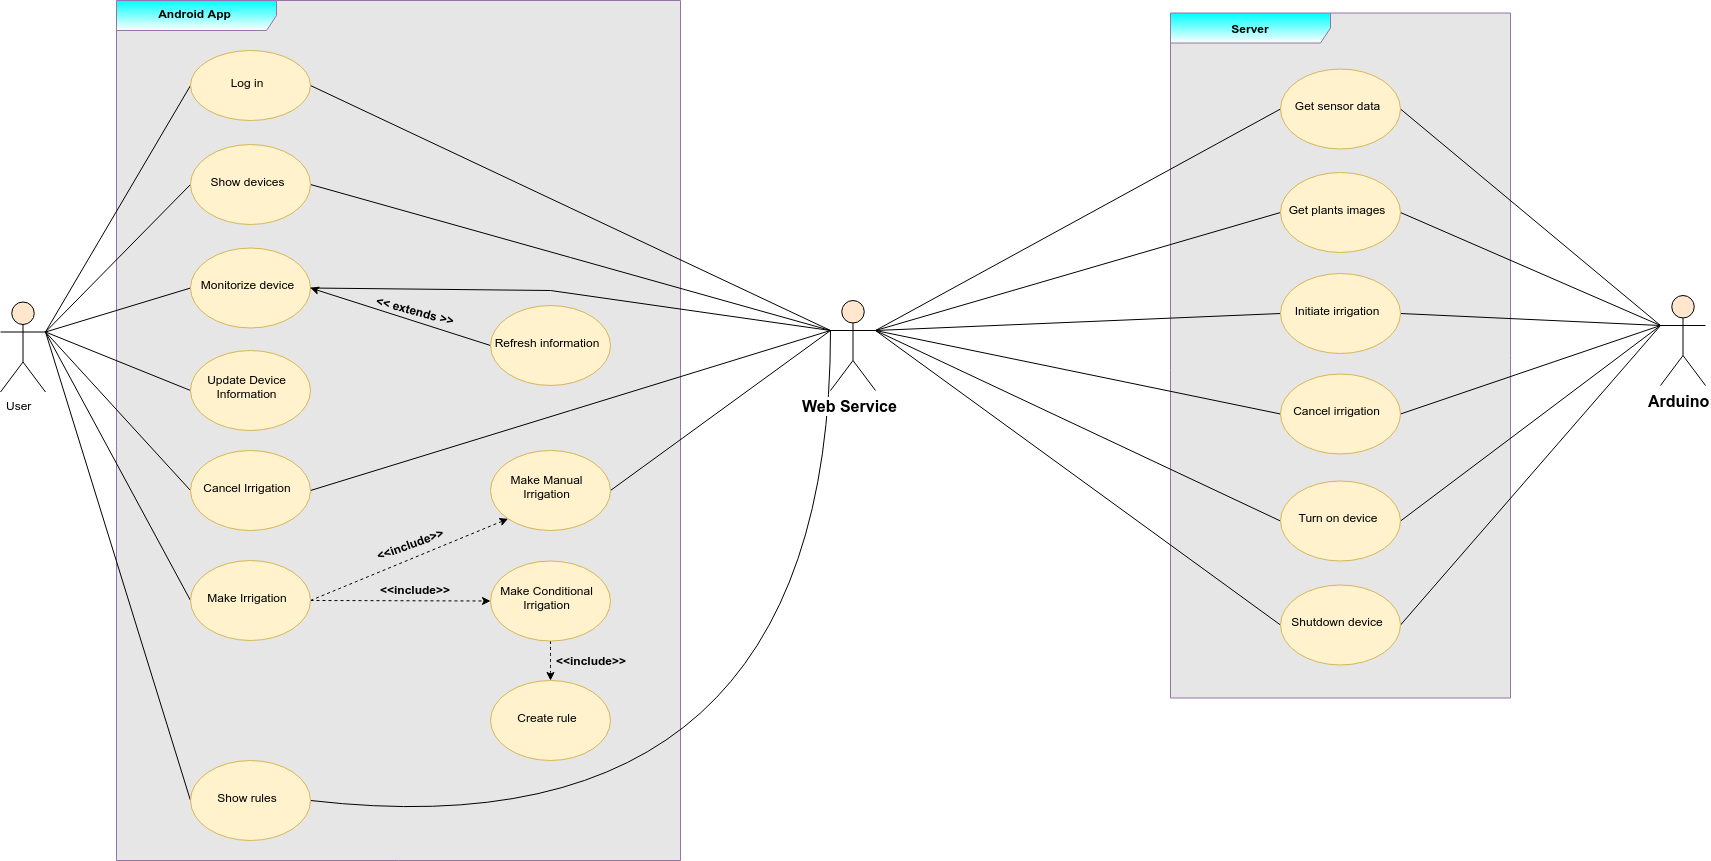
\includegraphics[scale=0.3195,angle=90,origin=c]{figures/usecasediagram.png}
\caption{Application use cases diagram}
\end{figure}

\newpage

\section{General architecture}
\subsection{System architecture}
\begin{figure}[hbtp]
\centering
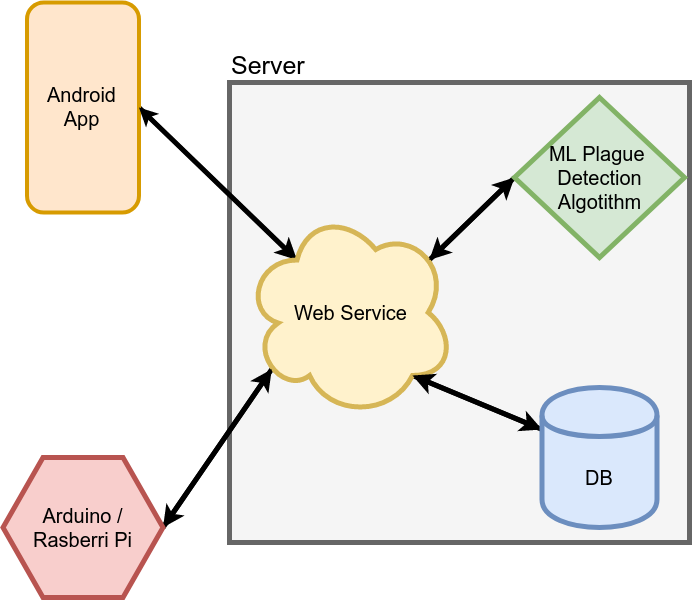
\includegraphics[scale=0.6]{figures/AppArchitecture.png}
\caption{System app architecture}
\end{figure}

La arquitectura de nuestra applicación está compuesta por:
\begin{itemize}
\item \textbf{Android App}: Interfície gráfica, encargada de recopilar los datos introducidos por el usuari.
\item \textbf{Web Service}: Hace de middleware de la aplicación. Se encarga de gestionar las peticiones entre la app Android y el Arduino/Raspberry pi, la base de datos, ...
\item \textbf{Arduino/Raspberry pi}
\end{itemize}

\newpage

\subsection{Arduino/Raspberry pi architecture}
\begin{figure}[hbtp]
\centering
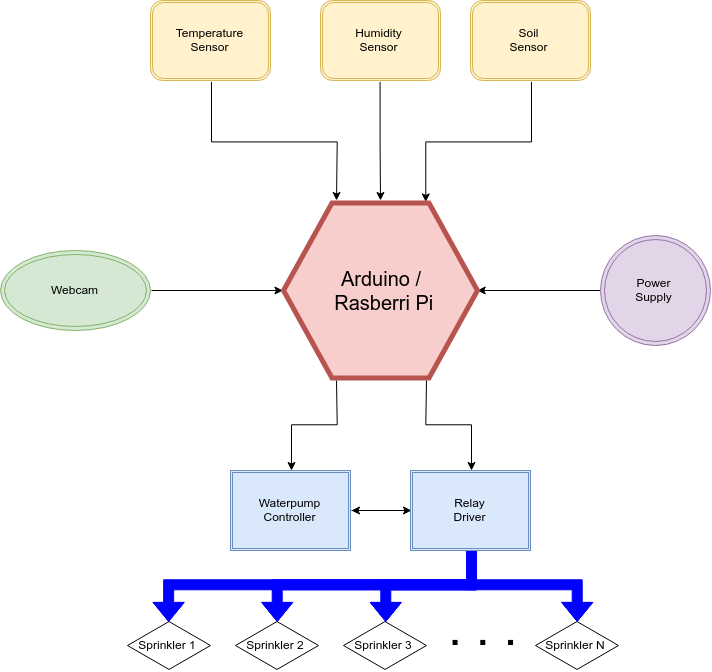
\includegraphics[scale=0.6]{figures/ArduinoArch.png}
\caption{Arduino and rapsberry pi architecture}
\end{figure}

\newpage

\section{Data model}
%% Data model
\begin{figure}[hbtp]
\centering
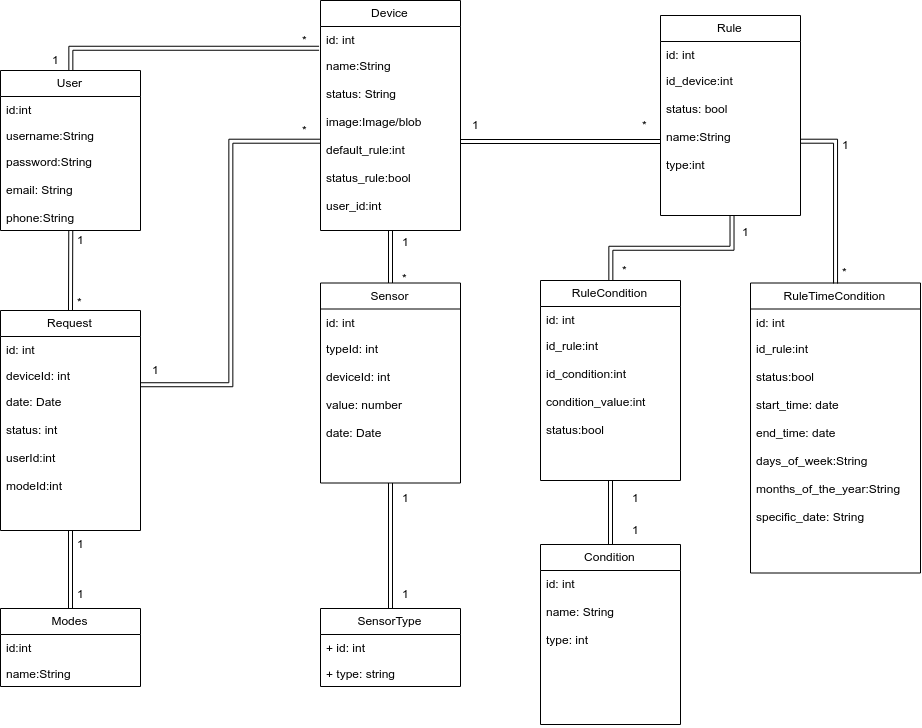
\includegraphics[scale=0.5]{figures/ModelDeDades.png}
\caption{Data model UML}
\end{figure}

\section{Product backlog}
%% User stories
\begin{center}
\begin{adjustbox}{angle=90,width=2.9in}
\begin{tabular}{|l|l|l|l|l|l|}
\hline
\textbf{Id} & \textbf{As a} & \textbf{I want to be able to} & \textbf{So that} & \textbf{Priority} & \textbf{Sprint} \\
\hline \hline
1 & User & Change the app language & I can visualize the content in some other languages & MEDIUM & 1 \\
\hline
2 & User & Visualize all the app screens & I can navigate throught all screens & HIGH & 1 \\
\hline
3 & User & Log in into the app & I can use the app functionalities & LOW & 2 \\
\hline
4 & User & Visualize the sensor characteristics of my plants & I can decide the best moment to irrigate & MEDIUM & 2 \\
\hline
5 & User & Activate or deactivate my devices & I can disconnect or connect my device & MEDIUM & 2 \\
\hline
6 & User & Create rules for each device & I can manage my plants automatically & MEDIUM & 2 \\
\hline
7 & User & Create conditions for each rule & I can establish more than one condition to activate the rule & MEDIUM & 2 \\
\hline
8 & Admin & View all users available & I can control the app access & LOW & 3 \\
\hline
9 & User & Irrigate manually from one device & I can irrigate my plants whenever i want & MEDIUM & 3 \\
\hline
10 & User & Visualize if my plants are infected & I can treat the infection as soon as possible & MEDIUM & 3 \\
\hline
11 & User & Irrigate automatically using rules and conditions & I can not worry about when to irrigate & MEDIUM & 3 \\
\hline
12 & User & Modify my device profile & I can change the image and the device name & LOW & 3 \\
\hline
13 & User & Update or delete the rules and conditions & I can modify my rules & MEDIUM & 3 \\
\hline
14 & Admin & Create, modify and delete users from the database & I can modify user into the database & MEDIUM & 4 \\
\hline
15 & Admin & Create, modify and delete devices associated with an user & I can modify devices into de database & MEDIUM & 4 \\
\hline
16 & Admin & Monitorize the cpu traffic and current device status & I can make user support (helpdesk) & LOW & 4 \\
\hline
\end{tabular}
\end{adjustbox}
\end{center}

\newpage

\section{Sprint backlog + dedication to each one}
%% Sprint backlog + dedication to each one

\section{Main screens desgin mockup}
%% Main screens desgin mockup
\begin{itemize}
\item Link: \url{https://marvelapp.com/5bj64b2/screen/62745623}
\end{itemize}

\newpage

\section{Navigation schema between activities}
%% Navigation schema between activities

\section{Economic viability}
\subsection{Who?}
%% multi/single Sector, Interest, Geographically, Size of organization
%% Type of clients, sector, ...

\subsection{How many?}
%% Periods (year, month..), Per sector?, Per customer type?
	
\subsection{Strategy}
%% Marketing campaigns, Ads, door-to-door / Demos , ‘Word-to-mouth’
%% App Costs. Monetization strategy

\end{document}